
\section{Evaluation Metrics}

As already described in Section \ref{sec:validation}, we have collected several metric indicator to pick the best models among the cross-validated ones.

The two following tables display the averaged metrics resulted from cross-validation, complete with standard deviation, separating results from \textbf{overall assessment} and \textbf{full-tumor assessments}.

\begin{table}[H]
\centering
\begin{tabular}{|c|c|c|c|c|}
\hline 
& \textbf{A1} & \textbf{A2} & \textbf{I1} & \textbf{I2}
\\ \hline \hline
\textbf{Acc.} & $0.9125 \pm 0.0044$ & \textcolor{mygreen}{$0.9172 \pm 0.0031$} & \textcolor{myred}{$0.8966 \pm 0.0058$} & $0.9041 \pm 0.0048$
\\ \hline
\textbf{Prec.} & $0.9100 \pm 0.0071$ & \textcolor{myred}{$0.8948 \pm 0.0064$} & \textcolor{mygreen}{$0.9138 \pm 0.0066$} & $0.9122 \pm 0.0069$
\\ \hline
\textbf{Spec.} & $0.6084 \pm 0.0163$ & \textcolor{myred}{$0.5458 \pm 0.0102$} & $0.6549 \pm 0.0156$ & \textcolor{mygreen}{$0.6590 \pm 0.0106$}
\\ \hline
\textbf{Sens.} & $0.9552 \pm 0.0069$ & \textcolor{mygreen}{$0.9822 \pm 0.0015$} & \textcolor{myred}{$0.9338 \pm 0.0068$} & $0.9449 \pm 0.0042$
\\ \hline
\textbf{IoU} & $0.8929 \pm 0.0063$ & \textcolor{mygreen}{$0.9019 \pm 0.0043$} & \textcolor{myred}{$0.8762 \pm 0.0075$} & $0.8854 \pm 0.0062$
\\ \hline
\textbf{F1} & $0.9414 \pm 0.0037$ & \textcolor{mygreen}{$0.9471 \pm 0.0025$} & \textcolor{myred}{$0.9320 \pm 0.0044$} & $0.9377 \pm 0.0036$
\\ \hline
\end{tabular}
\caption{Overall validation metrics}
\end{table}

\begin{table}[H]
\centering
\begin{tabular}{|c|c|c|c|c|}
\hline
& \textbf{A1} & \textbf{A2} & \textbf{I1} & \textbf{I2}
\\ \hline \hline
\textbf{Acc.} & \textcolor{mygreen}{$0.9852$} & $0.9689$ & \textcolor{myred}{$0.7975$} & $0.8581$
\\ \hline
\textbf{Sens.} & \textcolor{mygreen}{$0.9852$} & $0.9689$ & \textcolor{myred}{$0.7975$} & $0.8581$
\\ \hline
\textbf{IoU} & \textcolor{mygreen}{$0.9852$} & $0.9689$ & \textcolor{myred}{$0.7975$} & $0.8581$
\\ \hline
\textbf{F1} & \textcolor{mygreen}{$0.9925$} & $0.9839$ & \textcolor{myred}{$0.8864$} & $0.9232$
\\ \hline
\end{tabular}
\caption{Full-tumor validation metrics}
\end{table}

\subsection{Overall Performances}

\par
From a general point of view, all models show some unbalanced results: while overall having high scores, they show unimpressive results regarding specificity, and, consequently, also F1 score. We can infer that the models has a \textbf{high chance of scoring false positive}; in other words, the models are likely to classify as tumor some areas that are not, disregarding some of the non-tumor regions. The other indicators show fairly high results because of the imbalances of the dataset: there's a great majority of tumor cells, so whenever the models mistakes a non-tumor nest for a tumor one, the overall accuracy is not significantly affected as non-tumor areas are in minority, but the indicator assessing the prediction quality over false classification is vastly worsened. 

\par
Despite the clear issue, it can be considered a minor problem in practice: our task is to develop techniques to highlight risks of tumor in pancreatic tissues, in order to show to experts who has authority on the subject to assess the actual health status of the patient and make informed decisions on how to operate. It is not our objective to develop a model able to pinpoint exactly, with absolute precision, the area of coverage of tumor and non-tumor cells. In other words, our models serves to ring a bell regarding the level of exposure to oncologic risk. Therefore, \textbf{it can be actually beneficial to have a system that is especially sensitive to tumors}, and is more susceptible to false positive, as it would be more prone to detect anomalies.

\par Besides that, we can also notice the sensibility and the F1 score are especially high, so \textbf{the models succeed in classifying positive true labels}, which is the indicator that carries more value in an a pathology detection problem such as ours.

\subsection{Differences Between Architectures}

\par
Besides the different training settings, \textbf{AlexNet tends to have better overall metrics} while actually having worse scores regarding the balance of class prediction quality, likely witnessing an higher imbalance than its adversary.

\par
At a first glance, indeed, Inception V3 scores higher for what concerns specificity, and, as a consequence, an F1 score as well. From this, we can understand that \textbf{Inceptions V3 addresses more effectively class imbalances}, underlining a greater robustness, while still achieving respectable results regarding other metrics indicator.

\par
Unfortunately, from what we can see in the second table, \textbf{AlexNet handles better full-tumor predictions}, being it more biased towards tumors. From this, we can understand that Inception V3 still has not effectively grasped the characteristics that separate one class from the other, despite performing better than AlexNet from this point of view.

\par To sum up, \textbf{AlexNet achieves better overall results}, but \textbf{Inception V3 show more balanced indicators}, while still delivering \textbf{similar performances}.

\subsection{Differences Between Training Settings}

Training parameters affect the final results in a significant way:

\begin{itemize}
    \item \textbf{AlexNet}: \textbf{regularisation does not seem to help} with the prediction quality, as it slightly worsen the model's robustness, improving what was good about it but deepening its weaknesses. From this, we are persuaded to believe that \textbf{AlexNet does not over-fit}, as it has been stated in the original paper.

    \item \textbf{Inception V3}: leveraged to selectively address the trickier-to-handle non-tumor predictions, \textbf{focal loss actually harms the model's performance} from many perspectives. The standard cross-entropy training is to be preferred.
\end{itemize}

\section{Comparison with the Article}

Our study of the problem and the solution addressed to solve it go in different directions with respect to the paper:

\begin{itemize}
    \item AlexNet performs better than in the original article, achieving more robustness, especially less false positives, and does not over-fit.
    \item Inception  performs much worse, as it does score the excellent metrics shown in the paper. It is also much sensitive to class prediction imbalances, but, in analogy, it does not over-fit.
\end{itemize}

\section{Model Selection and Testing}

\par
In light of what has been said so far, we decided to select A1 and I2 out of the four validated, being them the ones delivering the most overall satisfying performances.

\par
At this point, we performed testing on them, to conclude the model assessment phase on another unbiased sample. The testing sample is the $29^{\text{th}}$ image, the last of the dataset, never used for training nor validation purposes, so completely new and unseen to the model as well as to us, to prevent any type of bias of ours.

\par
The following section illustrates the testing results and provides a comparison regarding the performance of the chosen models. The results of the models are always shown one next to each other, in order to ease visual comparisons.

\subsection{Testing Metrics}

\par
The following table collects the evaluation metrics computed on the testing image n. 29 for both selected models.

\begin{table}[H]
\centering
\begin{tabular}{|c|c|c|}
\hline
& \textbf{A1} & \textbf{I2}
\\ \hline \hline
\textbf{Acc.} & \textcolor{myred}{$0.9254$} & \textcolor{mygreen}{$0.9292$}
\\ \hline
\textbf{Prec.} & \textcolor{myred}{$0.9215$} & \textcolor{mygreen}{$0.9412$}
\\ \hline
\textbf{Spec.} & \textcolor{myred}{$0.5927$} & \textcolor{mygreen}{$0.7072$}
\\ \hline
\textbf{Sens.} & \textcolor{mygreen}{$0.9947$} & \textcolor{myred}{$0.9754$}
\\ \hline
\textbf{IoU} & \textcolor{myred}{$0.9170$} & \textcolor{mygreen}{$0.9194$}
\\ \hline
\textbf{F1} & \textcolor{myred}{$0.9567$} & \textcolor{mygreen}{$0.9580$}
\\ \hline
\end{tabular}
\caption{Selected models testing metrics}
\end{table}

We also provide the confusion matrix in two versions:
\begin{itemize}
    \item The first one shows the metrics w.r.t the number of classifications.
    \item The second one shows the metrics w.r.t the percentages of classifications.
\end{itemize}

\begin{figure}[H]
 \centering
 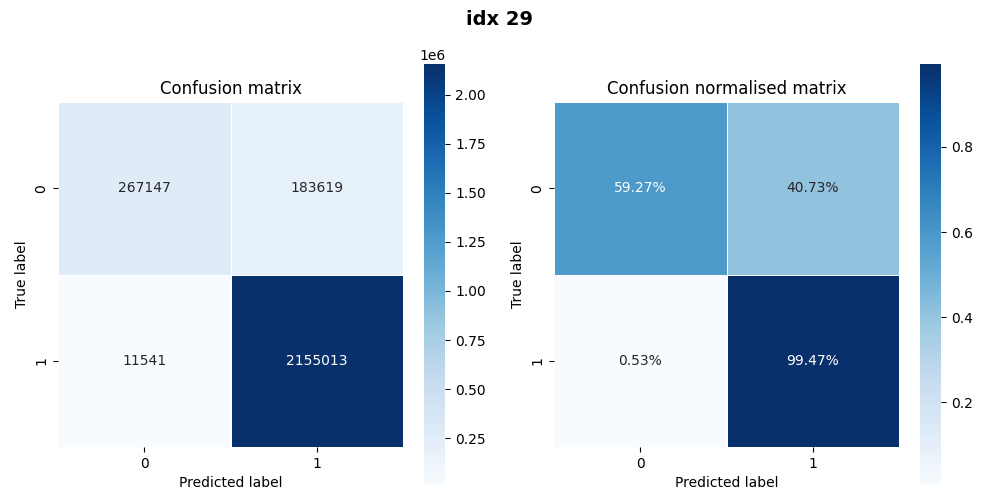
\includegraphics[scale=0.6, cframe=bluepoli 2pt]{./resources/A1_conf_matr_29.png}
 \caption[A1 test confusion matrix]
    {Testing confusion matrix of A1 predictions on image n. 29}
\end{figure}

\begin{figure}[H]
 \centering
 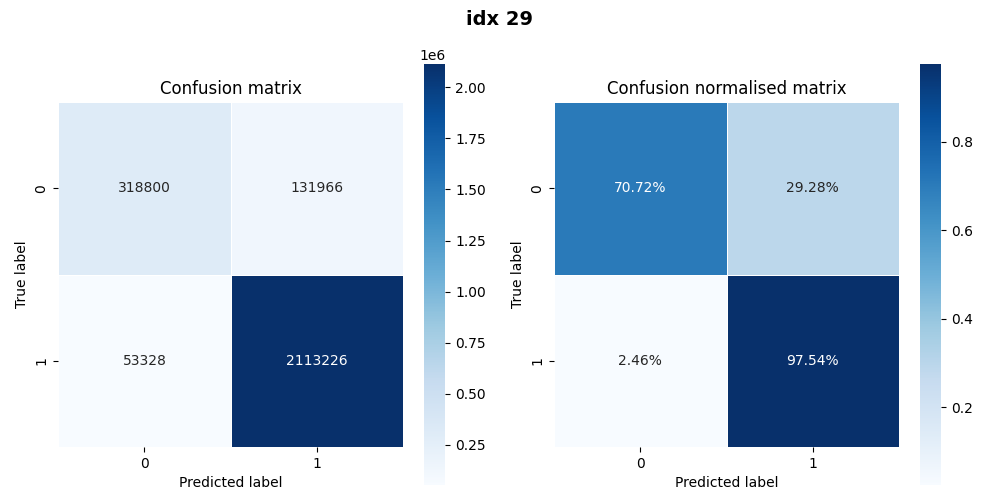
\includegraphics[scale=0.6, cframe=bluepoli 2pt]{./resources/I2_conf_matr_29.png}
 \caption[I2 test confusion matrix]
    {Testing confusion matrix of I2 prediction on image n. 29}
\end{figure}

As expected, in the context of this testing results, we can notice that the \textbf{two models behaved quite similarly} and that \textbf{I2 had a certain advantage in terms of prediction balance}. However, I2 performed slightly better, achieving marginally better scores in all indicators except sensitivity. Overall, the two models proved to deliver respectable and sufficiently reliable performances.

\subsection{Testing Visualisations}

\par
In this section, to conclude the testing procedure, we illustrate some of the visual artifact that allow us to judge by eye the behaviour of the two models.

\par
The prediction procedure on the testing image performed by the models produced the following binary probability mask:

\begin{figure}[H]
 \centering
 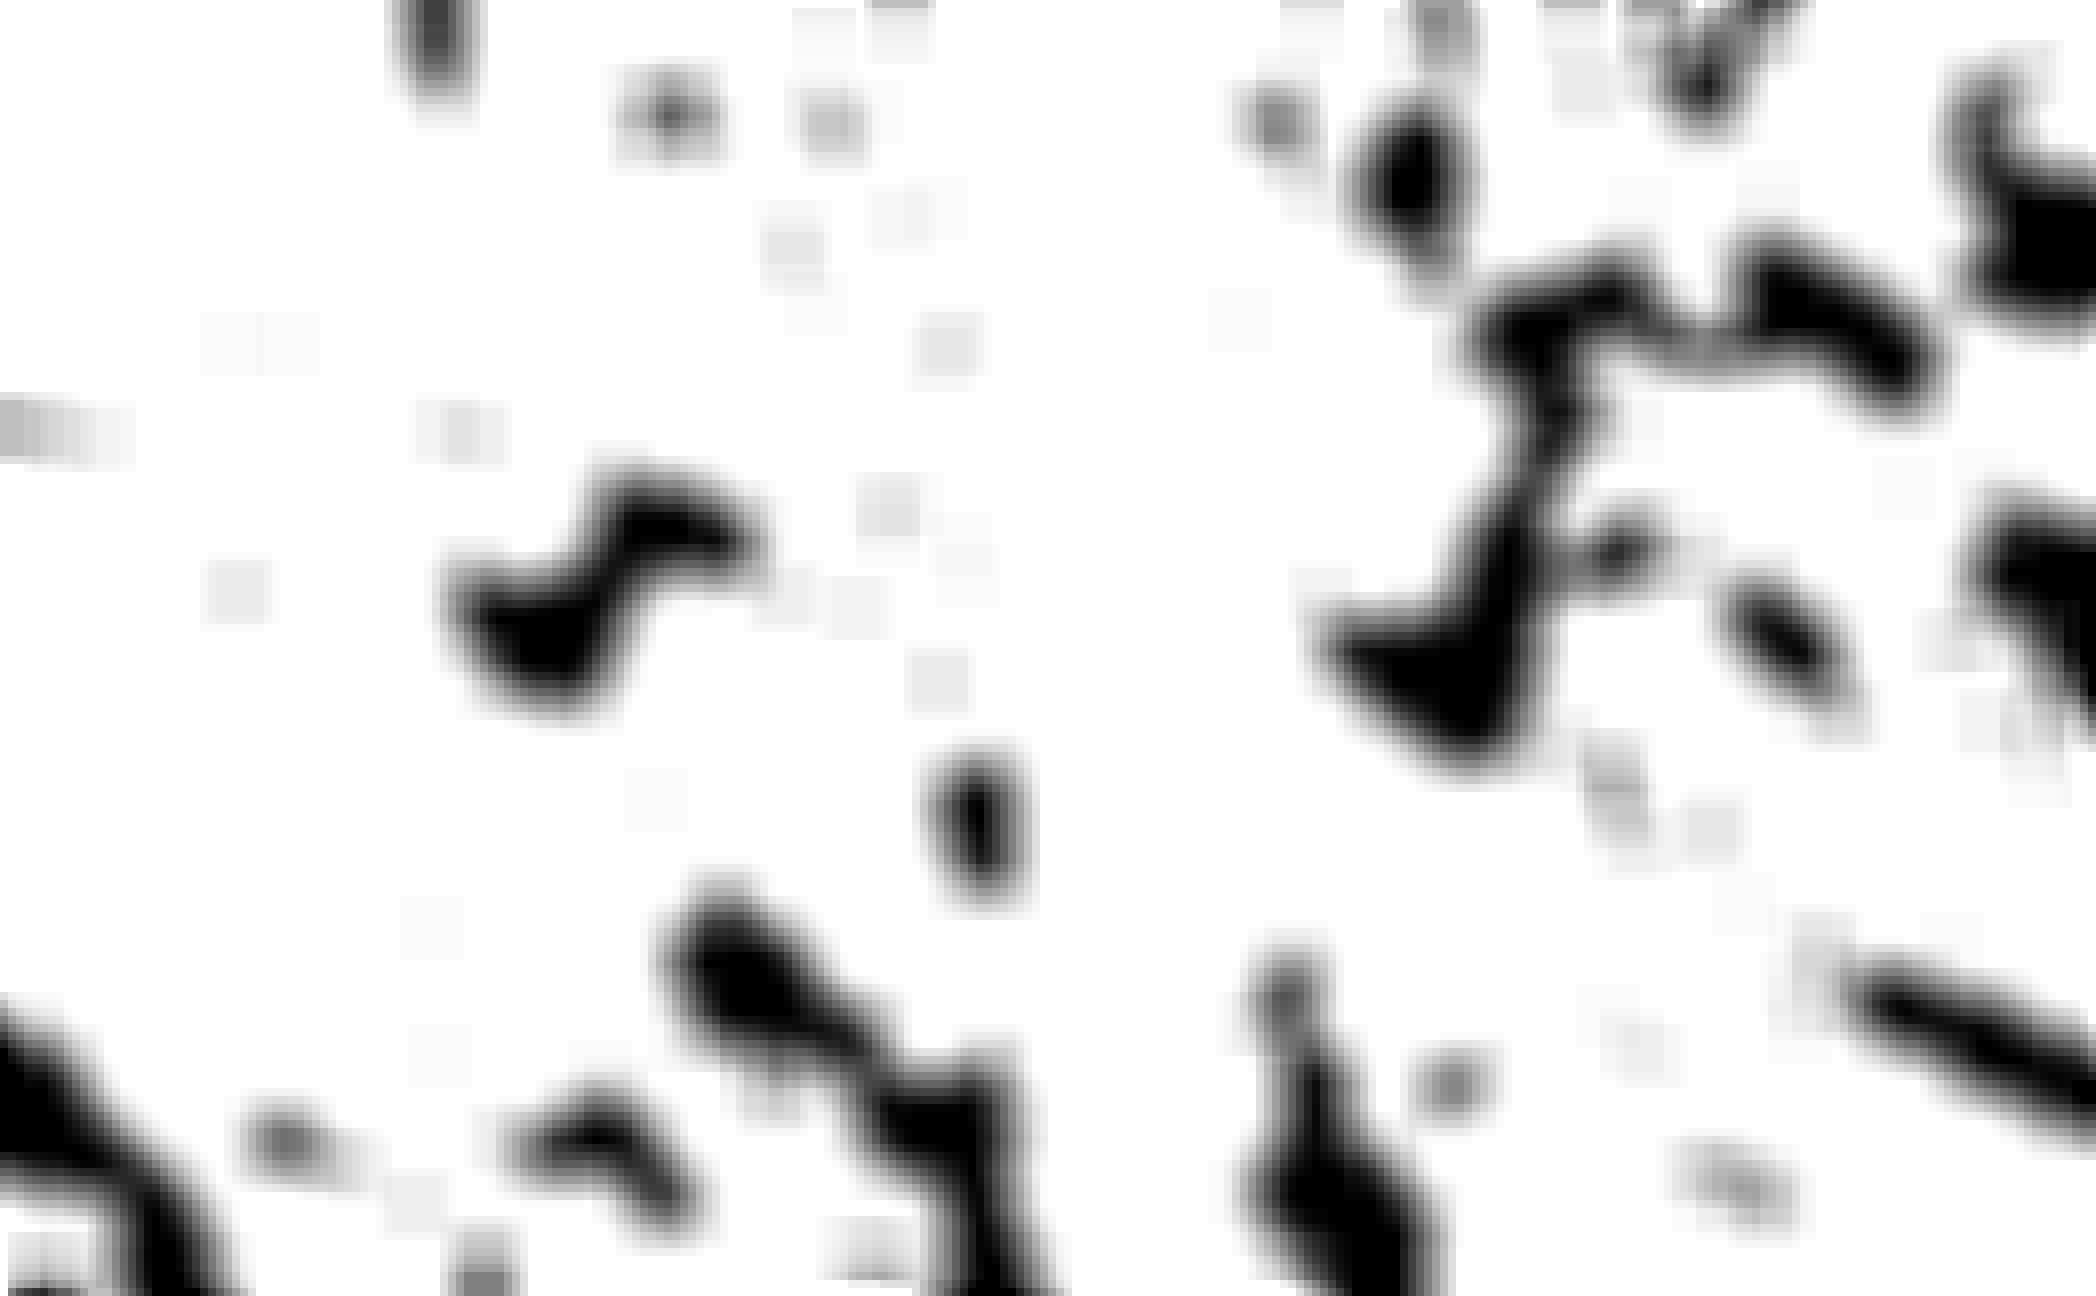
\includegraphics[scale=0.2, cframe=bluepoli 2pt]{./resources/A1_avg_29.png}
 \caption[A1 test prediction]
    {Testing prediction performed by A1 on image n. 29}
\end{figure}

\begin{figure}[H]
 \centering
 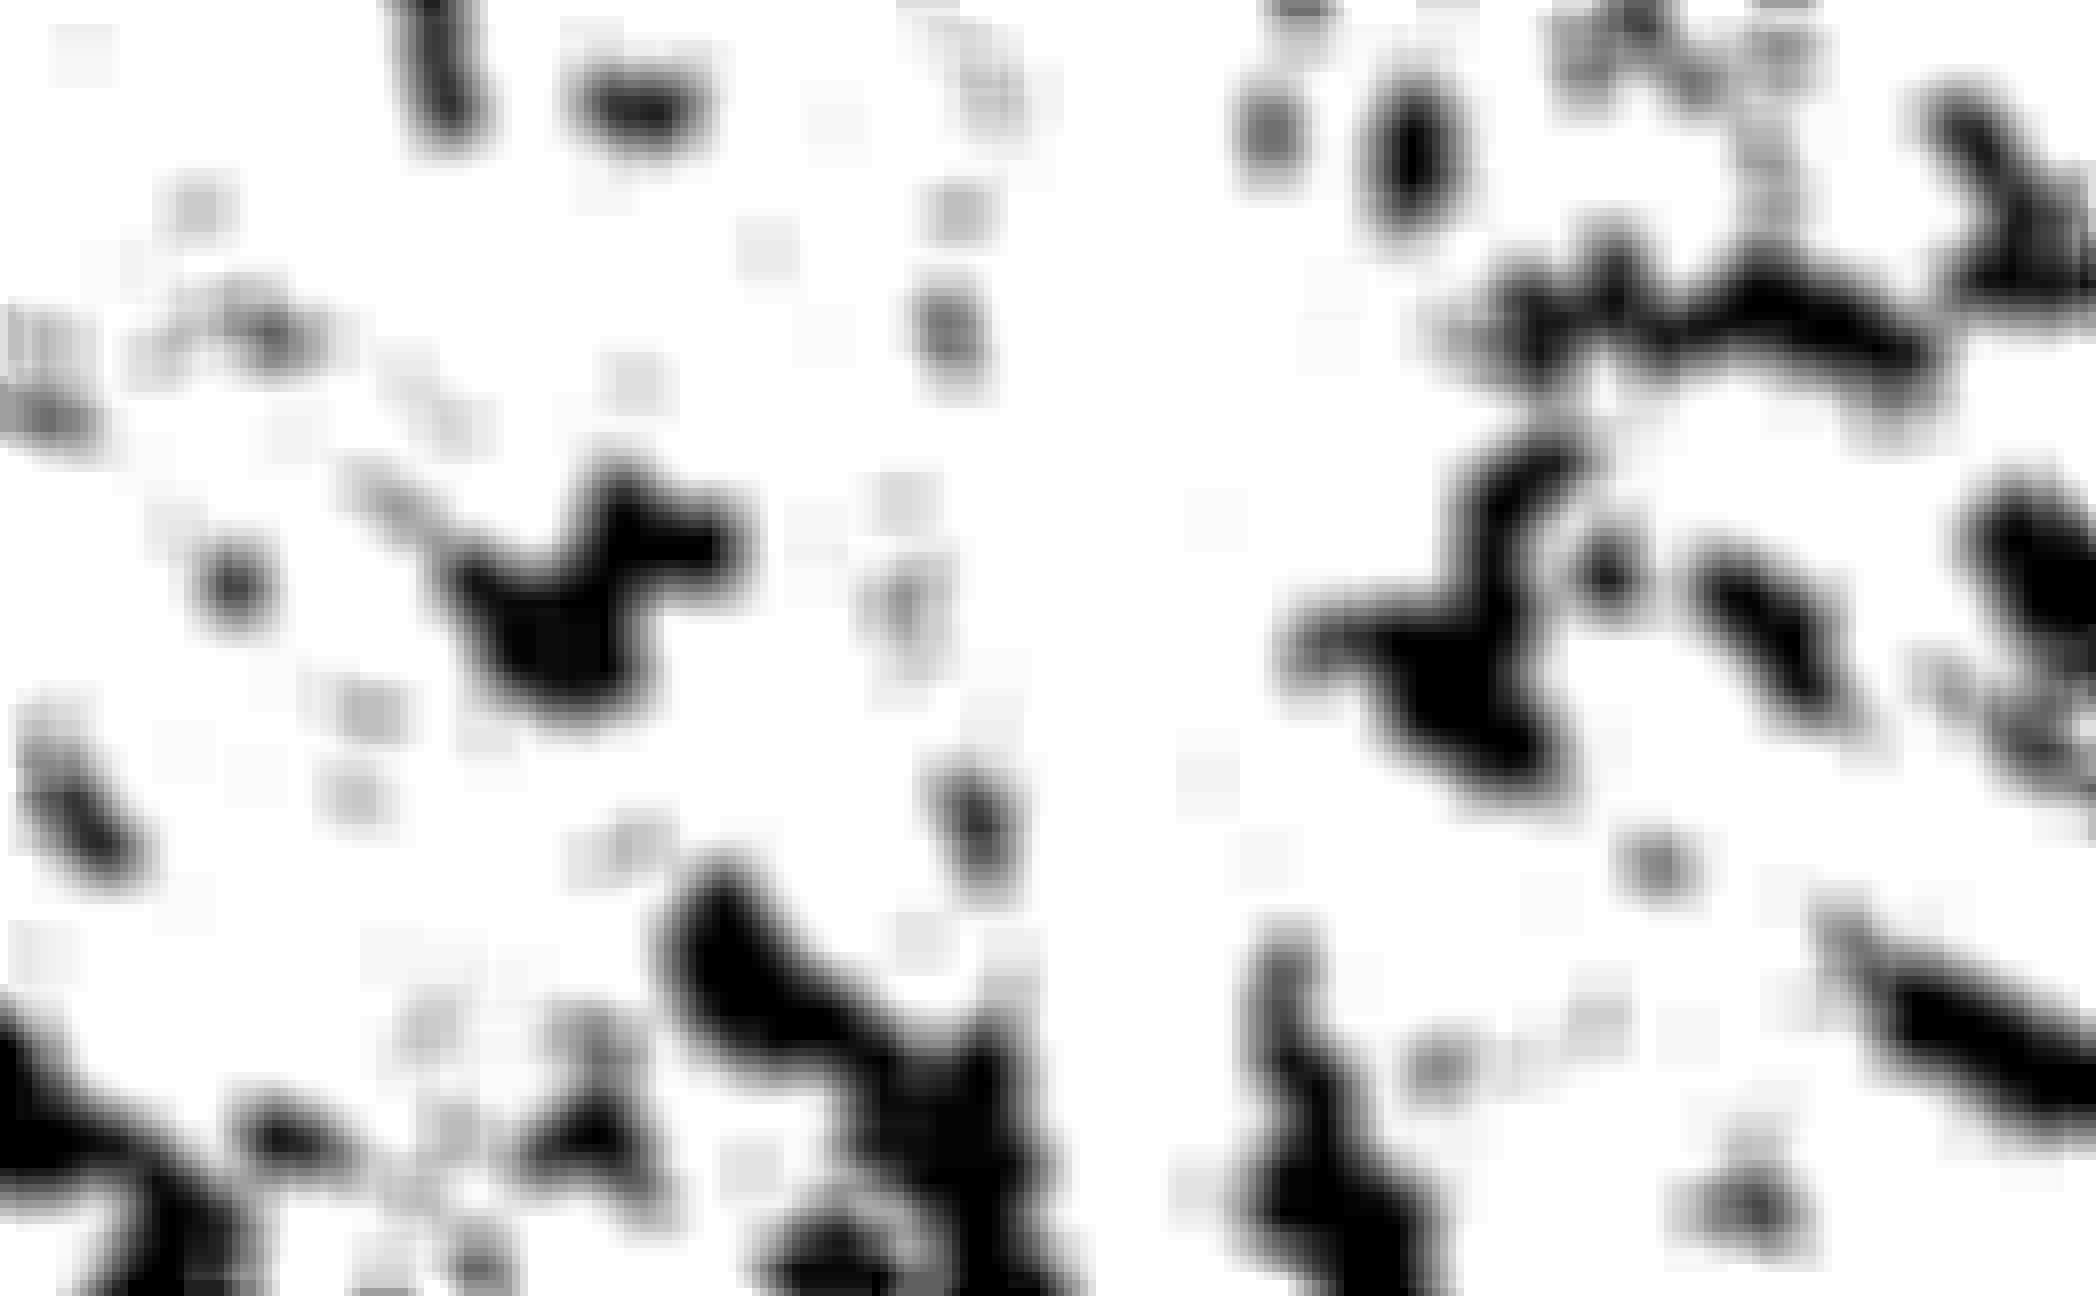
\includegraphics[scale=0.2, cframe=bluepoli 2pt]{./resources/I2_avg_29.png}
 \caption[A1 test prediction]
    {Testing prediction performed by I2 on image n. 29}
\end{figure}

\par
The mask, filtered to a threshold of 0.5, delivers our segmentation prediction:

\begin{figure}[H]
 \centering
 
\includegraphics[scale=0.2, cframe=bluepoli 2pt]{./resources/A1_pred_image_29.png}
 \caption[A1 thresholded test prediction]
    {Testing thresholded prediction performed by A1 on image n. 29}
\end{figure}

\begin{figure}[H]
 \centering
 
\includegraphics[scale=0.2, cframe=bluepoli 2pt]{./resources/I2_pred_image_29.png}
 \caption[I2 thresholded test prediction]
    {Testing thresholded  prediction performed by I2 on image n. 29}
\end{figure}

The following image shows a visual comparison between the predictions and the true segmentation mask available in the dataset, where:

\begin{itemize}
    \item White pixels are correct positive classifications.
    \item Black pixels are correct negative classifications.
    \item Green pixels are false positive classifications (Type 1 error).
    \item Red pixels are false positive classifications (Type 2 error).
\end{itemize}

\begin{figure}[H]
 \centering
 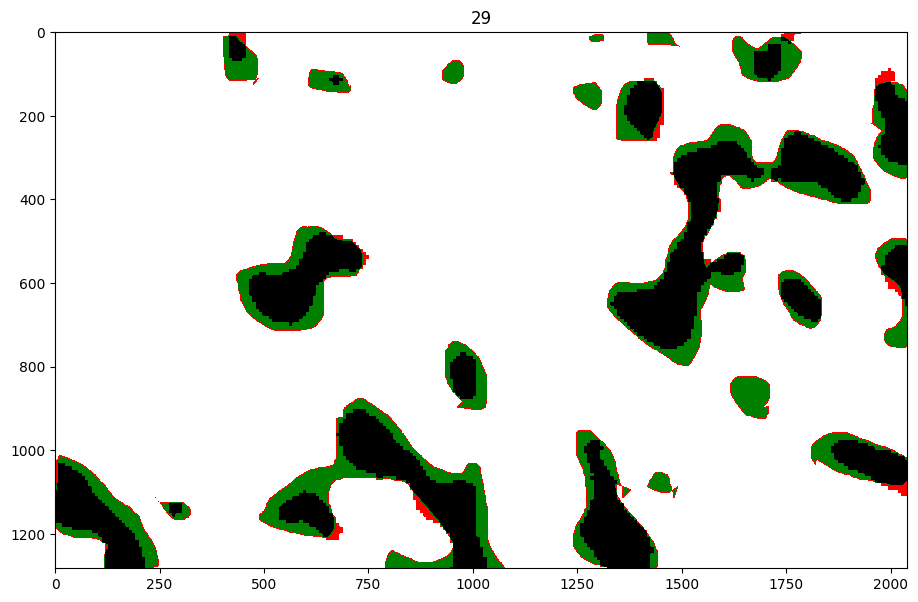
\includegraphics[scale=0.6]{./resources/A1_comp_29.png}
 \caption[A1 test prediction comparison]
    {Visual comparison of prediction performed by A1 on image n. 29 with true mask}
\end{figure}

\begin{figure}[H]
 \centering
 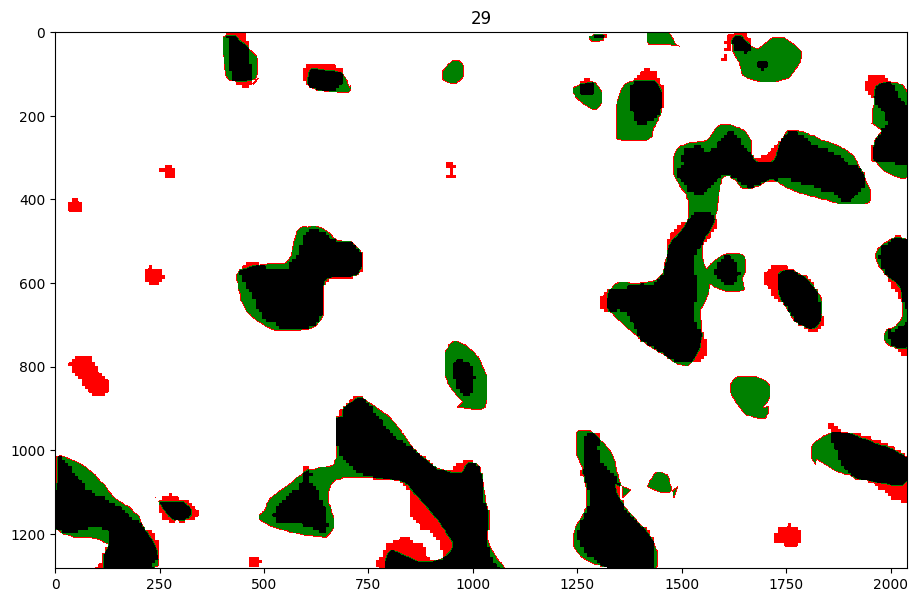
\includegraphics[scale=0.6]{./resources/I2_comp_29.png}
 \caption[I2 test prediction comparison]
    {Visual comparison of prediction performed by I2 on image n. 29 with true mask}
\end{figure}